\documentclass[11pt,a4paper,english]{article}
\usepackage{geometry,dtklogos,hyperref,babel,mdwlist,array,multicol}
\usepackage[default,osf]{sourcesanspro}
\usepackage[scaled=.95]{sourcecodepro}

\hypersetup{
    colorlinks,
    citecolor=blue,
    filecolor=blue,
    linkcolor=blue,
    urlcolor=blue
}
\newcommand*\file[1]{\href{run:#1.pdf}{#1}}

\title{\bfseries
	\Huge sourcesanspro\\
	\Large Adobe's Source Sans Pro typeface for \LaTeX
}

\author{Silke Hofstra, \href{mailto:tex@slxh.nl}{tex@slxh.nl}}
\date{Documentation for sourcesanspro v2.5.\\ \today}

\begin{document}
\maketitle
\begin{multicols}{2}
This package provides the Source Sans Pro font in an easy to use way. For \XeLaTeX\ and \LuaLaTeX\ users the original OpenType fonts are used. The entire font family is included. It can also be downloaded from \href{https://github.com/adobe/source-sans-pro}{Github}.

\section{Options}
The package has the following options:
\begin{itemize*}
	\item \textbf{oldstyle, osf}:  use old style numbers.
	\item \textbf{lining, nf, lf}: use lining numbers.
	\item \textbf{tabular}:        use fixed-width numbers.
	\item \textbf{proportional}:   use normal numbers.
	\item \textbf{black}:          \texttt{\textbackslash bfseries} is black.
	\item \textbf{semibold}:       \texttt{\textbackslash bfseries} is semibold.
	\item \textbf{bold}:           \texttt{\textbackslash bfseries} is bold.
	\item \textbf{light}:          \texttt{\textbackslash mdseries} is light.
	\item \textbf{extralight}:     \texttt{\textbackslash mdseries} is extra light.
	\item \textbf{regular}:        \texttt{\textbackslash mdseries} is regular.
	\item \textbf{scale, scaled}:  Change the scaling with a factor. For example:  \texttt{scale=.5}
	\item \textbf{default}:        Source Sans Pro is set as the default font family and as the sans serif family.
	\item \textbf{nosfdefault}:    Source Sans Pro is not set as sans-serif family.
	\item \textbf{type1, t1}:      Override automatic detection and use the Type 1 fonts.
	\item \textbf{opentype, otf}:  Override automatic detection and use OpenType fonts.
\end{itemize*}
The following options are enabled by default: lining, proportional, bold and regular.

\section{Commands}
Commands for all weights are also provided for \XeLaTeX\ and \LuaLaTeX\ users.
\begin{itemize*}
	\item \texttt{\bfseries \textbackslash sourcesanspro}
		-- the regular and bold weights.
	\item \texttt{\bfseries \textbackslash sourcesansprolight}
		-- the light and semibold weights.
	\item \texttt{\bfseries \textbackslash sourcesansproextreme}
		-- the extra light and black weights.
\end{itemize*}

\section{Licence}
Adobe's Source Sans Pro typeface is available under the \href{http://scripts.sil.org/OFL}{SIL Open Font License 1.1}.\\
All \LaTeX\ code is available under the \href{http://www.latex-project.org/lppl/}{\LaTeX\ project public license} v1.3 or later.

\section{Specimen}
Simple specimen can be found on page \pageref{sec:specimen}. Full specimen can be \href{http://store1.adobe.com/type/browser/pdfs/1959.pdf}{acquired from Adobe}.

\section{OpenType}
The OpenType fonts have many features, including old style numerals (1 6 9),  ligatures (ff fi fl ft {\addfontfeature{Style=Alternate}fl}) and stylistic alternatives ({\addfontfeature{Style=Alternate} l a g I}).

\subsection{Features}
A complete list of available font features is available on page \pageref{sec:otfinfo}. More information on how to use font features can be found in the \href{http://mirror.ctan.org/macros/latex/contrib/fontspec/fontspec.pdf}{fontspec documentation}.

\subsection{Files}
\begin{itemize*}
	\item SourceSansPro-ExtraLight.otf
	\item SourceSansPro-ExtraLightIt.otf
	\item SourceSansPro-Light.otf
	\item SourceSansPro-LightIt.otf
	\item SourceSansPro-Regular.otf
	\item SourceSansPro-RegularIt.otf
	\item SourceSansPro-Semibold.otf
	\item SourceSansPro-SemiboldIt.otf
	\item SourceSansPro-Bold.otf
	\item SourceSansPro-BoldIt.otf
	\item SourceSansPro-Black.otf
	\item SourceSansPro-BlackIt.otf
\end{itemize*}

\section{Type1}
The following Type1 font families are included:
\begin{itemize*}
	\item SourceSansPro-LF
	\item SourceSansPro-TLF
	\item SourceSansPro-OsF
	\item SourceSansPro-TOsF
\end{itemize*}
With series ‘el’, ‘l’, ‘m’, ‘sb’, ‘b’, ‘k’ and shapes ‘n’, ‘i’ and ‘sc’.

\section{Version history}
\subsection*{2.5}
\begin{itemize*}
	\item Updated fonts to 2.010
\end{itemize*}

\subsection*{2.4}
\begin{itemize*}
	\item Fixed errors in weight implementation.
	\item Updated fonts to 1.065
\end{itemize*}

\subsection*{2.3}
\begin{itemize*}
	\item Weights are now handled with the \href{http://www.ctan.org/pkg/mweights}{mweights} package.
\end{itemize*}

\subsection*{2.2}
\begin{itemize*}
	\item Updated fonts to 1.050
	\item Added \texttt{nosfdefault} option.
\end{itemize*}

\subsection*{2.1}
\begin{itemize*}
	\item Updated fonts to 1.040
\end{itemize*}

\subsection*{2.0}
\begin{itemize*}
	\item Merged all \texttt{.sty} files into \texttt{sourcesanspro.sty}.
	\item \texttt{default} option now sets the default font family to \texttt{Source Sans Pro}, not \texttt{\textbackslash sfdefault}.
	\item \texttt{type1}, \texttt{t1}, \texttt{opentype} and \texttt{otf} option added to override automatic detection.
	\item Added \texttt{OT1} to \texttt{fontspec} options.
\end{itemize*}

\subsection*{1.02}
\begin{itemize*}
	\item Changed the order of \texttt{T1} and \texttt{LY1}.
	\item Changed \texttt{lining}/\texttt{nf} behaviour.
	\item Redefined \texttt{\textbackslash oldstylenums}.
\end{itemize*}

\section{Known issues}
\begin{itemize*}
	\item Using \texttt{\textbackslash liningnums} when the default numbers are oldstyle results in an ‘font feature does not exist’ error and no lining numbers due to lack of the ‘lnum’ font feature.
\end{itemize*}

\newpage
\end{multicols}

\section{Specimen}
\label{sec:specimen}
\subsection{OpenType}
\begin{figure}[ht]
	\centering
	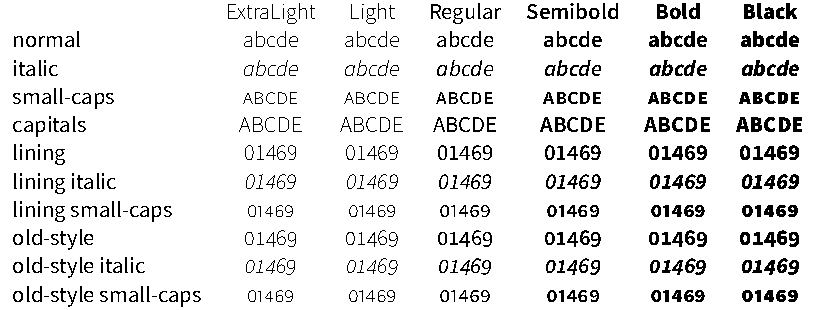
\includegraphics{sourcesanspro-otf-specimen}
\end{figure}
This table can also be found in \file{sourcesanspro-otf-specimen}.

\subsection{Type1}
\begin{figure}[ht]
	\centering
	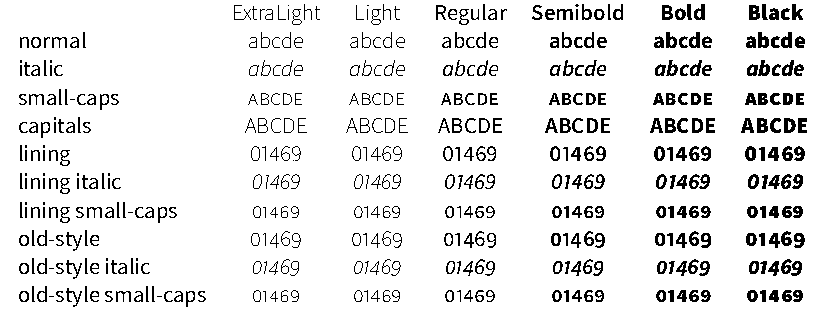
\includegraphics{sourcesanspro-type1-specimen}
\end{figure}
This table can also be found in \file{sourcesanspro-type1-specimen}.

\newpage
\section{Opentype features}
\label{sec:otfinfo}

\begin{figure}[ht]
	\centering
	\begin{tabular}{>{\ttfamily}l l}
		aalt & Access All Alternates \\
		c2sc & Small Capitals From Capitals \\
		case & Case-Sensitive Forms \\
		ccmp & Glyph Composition/Decomposition \\
		dnom & Denominators \\
		frac & Fractions \\
		kern & Kerning \\
		liga & Standard Ligatures \\
		mark & Mark Positioning \\
		mkmk & Mark to Mark Positioning \\
		numr & Numerators \\
		onum & Oldstyle Figures \\
		ordn & Ordinals \\
		pnum & Proportional Figures \\
		salt & Stylistic Alternates \\
		sinf & Scientific Inferiors \\
		size & Optical Size \\
		smcp & Small Capitals \\
		ss01 & Stylistic Set 1 - alternate l \\
		ss02 & Stylistic Set 2 - alternate a \\
		ss03 & Stylistic Set 3 - alternate g \\
		ss04 & Stylistic Set 4 - alternate I \\
		%ss05 & Stylistic Set 5 \\
		subs & Subscript \\
		sups & Superscript \\
		zero & Slashed Zero
	\end{tabular}
\end{figure}
\textit{(list generated with otfinfo)}

\end{document}

